\documentclass{scrartcl}
\usepackage{multicol}
\usepackage{epigraph}
\usepackage{url}
\usepackage{listings}
\usepackage{graphicx}
\usepackage{color}
\usepackage[parfill]{parskip}
\usepackage{titlesec}
\usepackage{geometry}
\usepackage{todonotes}
\usepackage{hyperref}
\usepackage{booktabs}
\usepackage{longtable}
\usepackage{array}

\lstset{
breaklines=true,
breakautoindent=true,
postbreak=\space,
tabsize=2,
basicstyle=\ttfamily\footnotesize,
showspaces=false,
showstringspaces=false,
extendedchars=true,
}

\newcommand{\horizontalrule}[1]{\rule{\linewidth}{#1}}
\def\changemargin#1#2{\list{}{\rightmargin#2\leftmargin#1}\item[]}
\let\endchangemargin=\endlist

\newcounter{savepage}

\setlength{\LTleft}{0pt}

\title{\horizontalrule{1pt}\\[0.5cm]Large-scale drive-by download detection: visit$^n$. process. analyse. report.}
\subtitle{Master in System and Network Engineering \\[0.5cm] \horizontalrule{1pt} }
\author{}
\date{}

\begin{document}
\pagenumbering{gobble}
\newgeometry{top=4cm,bottom=1cm}

\centerline{\includegraphics[width=10cm]{Images/UvA-logo-english}}

\begin{center}
\horizontalrule{1pt}\\[0.5cm]
\usekomafont{title}{\huge Large-scale drive-by download detection: \\[0.2cm] visit$^n$. process. analyse. report.}
\\[0.1cm]
\usekomafont{subtitle}{Master in System and Network Engineering} \\[0.5cm]
\horizontalrule{1pt} 
\end{center}

\vspace{7cm}

\begin{center}

\Large
Students:\\[0.5cm]

\begin{minipage}{0.4\textwidth}
\begin{flushleft} \Large
Adriaan Dens\\\texttt{adriaan.dens@os3.nl}
\end{flushleft}
\end{minipage}%
\begin{minipage}{0.4\textwidth}
\begin{flushright} \Large
Martijn Bogaard\\\texttt{martijn.bogaard@os3.nl}
\end{flushright}
\end{minipage}\\[1.6cm]

\Large
Supervisors:\\[0.5cm]

\begin{minipage}{0.4\textwidth}
\begin{flushleft} \Large
Jop van der Lelie\\\texttt{jop.vanderlelie@ncsc.nl}
\end{flushleft}
\end{minipage}%
\begin{minipage}{0.4\textwidth}
\begin{flushright} \Large
Wouter Katz\\\texttt{wouter.katz@ncsc.nl}
\end{flushright}
\end{minipage}\\[1.6cm]

{\Large \today}
\end{center}

\clearpage
\restoregeometry

\section*{Abstract}

Current malware analysis systems do not allow for concurrently visiting multiple websites. In this paper we present an algorithm which solves this problem by extensive monitoring of the environment. Additionally, a proof of concept has been developed which implements this algorithm. Results show a significant performance gain compared to current systems.

\clearpage

\tableofcontents

\clearpage

\pagenumbering{arabic}

\section{Introduction}

In the digital world of today, malware is still a massive and growing problem. While back in the day it was used to annoy users and system administrators, nowadays it's used for extortion, cyber espionage and surveillance by criminal groups and rivalling governments. One of the main risk factors to get infected with malware is a drive-by download while visiting a normal day-to-day website because, for example, the website got hacked and infected. 

In many cases\footnote{http://www.proofpoint.com/threatinsight/posts/malware-in-ad-networks-infects-visitors-and-jeopardizes-brands.php} \footnote{http://blog.fox-it.com/2013/08/01/analysis-of-malicious-advertisements-on-telegraaf-nl} \footnote{http://blog.fox-it.com/2014/01/03/malicious-advertisements-served-via-yahoo}, it was not the actual website but one of the advertisement networks that was infiltrated and which subsequently started serving malicious code hidden in innocently looking advertisement code. This is also called malvertising \cite{Li2012}.

National CERT organisations are interested in an early detection of such threats. While automated systems to scan websites already exist, like Cuckoo\footnote{http://cuckoosandbox.org} and Anubis\footnote{http://anubis.iseclab.org}, one of the main difficulties is the time needed to analyse a single website and the maintenance needed to keep these systems up-to-date for the latest threats.

The goal of this research project is to develop an algorithm that makes it possible to examine multiple websites for the existence of malware using the same computer system and at the same time. The effectiveness of this algorithm will be proven by implementing it in a proof of concept.

% Zeggen dat _wij_ dit en dat gaan doen om die en dat redenen

% Aanpassen aangezien we weten wat we hebben gedaan
% Mergen in introductie sectie

\subsection{Research Question}

In cooperation with the Dutch National Cyber Security Center (NCSC-NL), our research project will focus on the question:

\textit{How can we concurrently visit multiple URLs and still be able to determine which URL was responsible for malicious activities?}

To answer the research question, multiple sub-questions have been formulated:

\begin{itemize}
\item Which techniques are used by browsers to make concurrently visiting multiple URLs possible?
\item Which APIs are used by web browsers to make HTTP requests and retrieve webpages?
\item How can we link an HTTP request to its source URL without the modification of the used web browser?
\item What extra information from the client's (running) machine can be used to augment the information gained from network traffic to make the tracking of malware to its source URL easier?
\end{itemize}

% \subsection{Motivation?}

\subsection{Related work}

\todo{Referenties ombouwen naar 2 namen et al.}
The growing importance and economic losses of malware resulted in many research projects in the last years. The detection and analysis of malware has been researched from several different angles \cite{auto_malware,Chang2013} and resulted in many proposed static and dynamic analysis techniques.

In 2013, Le et al. \cite{Le2013} presented a framework that describes the common stages and characteristics of a drive-by download attack. They described four stages from placing the malicious content on a webpage until the execution of the malicious activity.

In 2011, a paper from Canali et al. \cite{Canali2011} was released about the problematic performance of dynamic analysis and with a solution proposed in the form of ``Prophiler''. Prophiler is a filter that deploys static analysis techniques and that is able to reduce the load with more than 85\% compared to dynamic analysis. This with a comparable amount of false negatives.

In the same year Rajab et al. \cite{Rajab11trendsin} gave an overview of the trends regarding web malware detection and how the malware tries to circumvent the detection. This research focused on the advantages and disadvantages of four techniques: Virtual Machine honeypots, Browser Emulation honeypots, Classification based on Domain Reputation and Anti-Virus Engines.

A different approach is taken by Rossow \textit{et al.} \cite{Rossow2011}, Cortjens \textit{et al.} \cite{Cortjens2012} and Kinkhorst \textit{et al.} \cite{Kinkhorst2009}. They have focused during multiple research projects on the ability to detect and identify malware on the network layer.

The usage of graphs to detect malware has been proposed before. Park and Reeves proposed\cite{Park2011} the usage of graphs of system calls to detect the similarities and difference in behaviour between the variations of a malware family. By focussing on the common subgraph, new variants can be detected and categorized without prior knowledge of their existence. A recent paper\cite{Wuchner2014} from W\"{u}chner \textit{et al.} described the usage of generating graphs from API calls for a heuristic based malware detection system.

The predecessor of NCSC-NL started in 2007 with the development of their own system, namely the Honeyspider network \cite{honeyspider}, for the dynamic analysis of websites. This system crawled the biggest and most important websites of the Netherlands on a daily base. The downside of this system is that it requires a lot of maintenance and hence it started to become outdated.

\iffalse
\subsection{Scope}

\todo{Zelfstandiger maken}

In this research project is an an algorithm created that allows multiple URLs to be opened at the same time while still being able to track all further interaction, such as unexpected HTTP requests and other malicious activity, and link them to the original request/URL. To prove that the algorithm is something feasible, a proof of concept of the algorithm has been implemented on top of the Cuckoo Sandbox.

The goal during this research project was to make the algorithm fully platform agnostic, however, several technical challenges prevented this. For this reason we limited our self to Windows 7 with version 8 of the Internet Explorer browser and have we the identified issues described.

The detection and identification of malicious behaviour was not part of this project. For our PoC we sticked to the detection of a well-known older and still to be determined malware family which existence is easy to detect on the system. 

\subsection{Ethical issues}

% Zinnen herschrijven die naar de toekomst verwijzen.
Our research contains no major ethical issues as it does not include working with personally identifiable information. Malware, if any, will be run in a controlled virtual environment. After every testrun the virtual machine will be automatically destroyed.

\fi


\clearpage

\section{Theory}
For a better insight into the project, it is nescesaary to introduce certain theoretical concepts first. In the next chapter this theory will be used to base the approach on for the design and development of the algorithm and choices regarding the proof of concept.

\subsubsection{Drive-by downloads}

\begin{figure}
    \centering
    \includegraphics[width=12cm]{Images/drive-by-download.png}
    \caption{The anatomy of a drive-by download malware infection. \cite{http://blog.armorize.com/2011/04/newest-adobe-flash-0-day-used-in-new.html (modified)}}
    \label{fig:dbdownload}
\end{figure}

\subsubsection{Behavior}

What will happen after a malware infection depends on the malware used and goals of the attacker. In many cases the malware will download further malicious components and nestle itself in the operating system so it will be restarted after a reboot of the operating system and be able to restore itself after an attempt to remove it.

To do this, the malware has to modify files, registery values and perform network operations. While in theory malware could directly communicate with the operating system kernel for this, most malware behaves like normal applications and use the installed or with the operating system provided libraries.

\subsection{API analysis}

In the early days were the libraries used by an application staticly linked into it. This means that the libraries becomes part of the application and it's no longer possible to determine which part of the application was originally part of the used libraries.

For performance and maintainability was dynamic linking invented. The application described which libraries it needs and the linker of the operating system will glue the applications and its dependent libraries together in the memoryspace of the application. 

Because the linker has to know all exported functions and where in the library it can found a function, a symbol table is part of every dynamic library. The same information can be used to hook into an provided function during runtime or to trick the linker to load a replacement of a certain function because the modified version has a higher priority.

This is called API hooking\cite{} and it's a very usefull technique to monitor the behavior of applications. The original function is then replaced by a substitute. This substitue functions calls for example the original function and logs the performed operation or is a custom replacement of the original function.

The technical implementation of API hooking is highly complex and platform specific and many different techniques\cite{http://jbremer.org/x86-api-hooking-demystified/} are possible. If the start of the application can be controlled, the linker search patch can be extended, a the replacement library stored somewhere in the searchpath or the import section of the application can be modified. When the application is already loaded or modification of the application or system is unwanted, the function to hook can be overwritten in memory with a replacement or jump to a different location in memory. However, this will prevent the ability to execute the original function unless the overwritten bytes are carefully preserved and reconstructed somewhere else.

In this project will API hooking be used to reverse engineer the internal working and API usage of web browsers and to log the behavior of malware for later analysis.

\subsection{Web browser architecture}
% Target: 4-6 blz

\todo{Meer bronnen?}

Modern web browsers are complex applications consisting of many components that have to work together. To develop a generic algorithm it is crucial to have first an in-depth insight in the working of the engines used to drive a web browser. In this project is focused on Internet Explorer, Mozilla Firefox, Chromium and Apple Safari. Those four browsers combined have a marketshare of more then 90\%\footnote{http://gs.statcounter.com/\#desktop-browser-ww-monthly-201412-201412-bar} \footnote{http://www.netmarketshare.com/browser-market-share.aspx?qprid=1\&qpcustomb=0}.

All modern web browsers allow the usage of multiple tabs with web pages in a single window. The underlying implementations differ creatly. In some browsers are only libraries provided by the operating system used while others decided to use their own. Also have some vendors decided to use multiple processes, sometimes even a new process for every single tab.

\textbf{Internet Explorer} is the well-known web browser from Microsoft. While until quite some time ago also a Mac version was available, in the last decade only the Windows version has been updated. Since version 7 is tabbed browsing available and version 8 was improved with the ability to run tabs from their own process (see figure \ref{fig:ie8proc}). This feature is called Loosely-Coupled IE\cite{http://blogs.msdn.com/b/ie/archive/2008/03/11/ie8-and-loosely-coupled-ie-lcie.aspx}. Every process runs independent from the other processes and runs its own network stack and instances of content plugins like Flash or Silverlight.

Starting each tab in its own process comes with an inevitable overhead by using more memory and the time it cost to start the process. For this reason can a process host multiple tabs. The amount of tabs to host in a single process and the maximum of processes to use is determined by the configuration. For backwards compatibility reasons is also the option provided to disable the usage of multiple processes and host all tabs in a single browser process.

The network stack used in Internet Explorer is provided by the Windows operating system and is called WinINet. This library provides high-level access to functions that allows applications to perform HTTP and FTP requests and utility functions for caching, proxys and security. After setting up the library and initiating and configuring the request, WinINet will perform the necessary steps to execute the request. WinINet depends for this on the Winsock library to setup the required network connections and Schannel to provide transparent support for SSL/TLS connections.

\begin{figure}
    \centering
    \includegraphics[width=9cm]{Images/IE8_process_model.png}
    \caption{The Internet Explorer process model starting from version 8. \cite{zelfde msdn link, modified}}
    \label{fig:ie8proc}
\end{figure}

\textbf{Firefox} is a cross-platform browser developed by the Mozilla foundation and one of the first that supported tabbed browsing. While it was first the main competitor for Internet Explorer, the release of Google Chrome made it lose some of its popularity.

In Firefox run only the plugins from a different process. The rendering of the web pages still happens from a single process. A long-term project to change that called Electrolysis\footnote{https://wiki.mozilla.org/Electrolysis} has been going on since 2009. In the new architecture is the entire rendering moved to a dedicated and sandboxed ``content'' process and is the main process used to host the user interface and serve as a proxy between the outside world and the content process. A longer-term goal is to spread the rendering of multiple tabs over more then one content process so that if a content process crashes not all tabs are affected.

To be platform independent is not directly interfaced with the provided libraries of the operating system. Instead a platform-neutral API called NSPR is used. Together with the NSS library that provides the functionality to create SSL/TLS connections is this used by the high-level network library called Necko. Necko provides the interface to perform HTTP and other protocol requests without revealing protocol, transport level or platform specific implementation details and is comparable to WinINet.

\textbf{Chromium} is the open-source version of the Google Chrome browser and is except a couple of proprietary components identical. While it's relative young, it is one of the most used web browsers. The big innovation of Chrome \cite{http://blog.chromium.org/2008/09/multi-process-architecture.html} was to use multiple processes instead of a single process. Besides its own process for every tab, have also the plugins and audio subsystem their own process. The subprocesses run in a sandbox with limited privileges and use the main process to communicate with the outside world.

\begin{figure}[h]
    \centering
    \includegraphics[width=9cm]{Images/Chrome_network.png}
    \caption{A high-level overview of the components involved in requesting an URL in Chromium. Platform specifics details related to sockets are hidden in StreamSocket and the usage of SSL/TLS is made transparent by using the interface-compatible SSLSocket instead of StreamSocket. \cite{http://www.chromium.org/developers/design-documents/network-stack, modified}}
    \label{fig:chrome_network}
\end{figure}

The library used by Chromium for network access is custom developed and tightly integrated in the engine. It provides similarly to Necko and WinINet a high-level interface (see figure \ref{fig:chrome_network}) but also it does contain lower level interfaces that interface directly with the operating system socket API. To provide transparent SSL/TLS support is the same library used as in Firefox, NSS.

\textbf{Safari} is the last browser that was examined in this project. It's the proprietary web browser of Apple that is since three years only available for their own operating system, Mac OS X. Around the same time\footnote{https://lists.webkit.org/pipermail/webkit-help/2011-July/002298.html} has support for using multiple processes been added. Safari is closed-source but build on top of many open-source components like JavaScriptCore and WebKit.

Safari uses until a certain limit a dedicated process for every tab. However for performance reasons and resource restrictions is after reaching the limit multiple tabs hosted in a single process. The network operations for the main and tab processes is concentrated in a dedicated process. Only this process will retrieve the webpages and use IPC mechanics to deliver the result to the correct process. 

CFNetwork is the library that is used by Safari for its network access. This library is one of the core frameworks of the OS X operating system and available for all applications. It provides interfaces for all relevant web related protocol. An unified interface called NSUrl like the other browsers use is also available, however because of the closed-source nature of Safari it's not possible without an extensive reverse engineering effort to determine if it's used instead of directly using the provided APIs of the CFNetwork library.

\iffalse

Which techniques are used by browsers to make concurrently visiting multiple
URLs possible?
	- Tabs of course
		- As a process
		- As multiple threads under the browser process

How can we link an HTTP request to its source URL without the modification of the used web browser?
we need extra information, see vraag 4
network is niet genoeg blablabla

How do web browsers make HTTP requests and retrieve webpages? Which Operating System level APIs are used?
	- Safari: CFNetwork and NSURLConnection(Loader) and IPC
		1 hoofdprocess: Safari
		1 process per tab: Safari Web Content
		1 process voor networking: Safari Networking
		Network stack of OS X.
	- Internet Explorer: C API calls naar Windows libraries
		Process per tab: is configureerbaar in settings/registry, je kan ook meerdere tabs in 1 process hebben
		Network stack of Windows
	- Firefox: C++ Library calls
		Single Process (+ 1 process voor flash)
		Own network stack Necko (nss3 voor trafiek te encrypten)
		\url{https://developer.mozilla.org/en-US/Firefox/Releases/3.5/Updating_extensions#Getting_a_load_context_from_a_request}
		http://stackoverflow.com/questions/10719606/is-it-possible-to-know-the-target-domwindow-for-an-httprequest
	- Chrome: IPC 
		1 hoofdprocess: Google Chrome die networking doet
		1 process per tab. (Altijd 13 threads?)
		1 process voor Flash.
		1 process voor Audio. (4 threads)
		Own network stack (nss3 voor trafiek te encrypten)
		http://www.chromium.org/developers/design-documents/network-stack

What extra information from the client's (running) machine can be used to augment the information gained from network trac to make the tracking of malware to its source URL easier?  
	- The Thread ID or Process ID van tabs, PDF reader, Java applet, ...
	- Handle bij IE
	- File descriptors
	- Process tree
	- Voordeel van op machine network traffic te intercepten is dat we rommel van andere applicaties niet zien, maar enkel het trafiek van de browser en de gespawnde subprocessen ervan.
	- 
\fi


\clearpage

\newgeometry{bottom=0.1cm}
\section{Approach and Methods}
%approach etc aan de handvan de rq's?

%\item Which techniques are used by browsers to make concurrently visiting multiple URLs possible?
%\item Which APIs are used by web browsers to make HTTP requests and retrieve webpages?
%\item How can we link an HTTP request to its source URL without the modification of the used web browser?
%\item What extra information from the client's (running) machine can be used to augment the information gained from network traffic to make the tracking of malware to its source URL easier?

Now the outline of this project has been set, it has become time to look how the research questions can be answered. 

\subsection{API analysis}

\subsection{Algorithm}
% Target: 3-4 blz

\begin{figure}[h]
    \centering
    \includegraphics[width=17cm]{Images/alg_tree.png}
    \caption{An example of the graph}
    \label{fig:alg_tree}
\end{figure}

\subsubsection{Design considerations}

\subsubsection{Generic algorithm}

- Disconnected DAGs

1) Hooker schrijven voor elke browser die trafiek tussen Netwerk en Browser of in de browser zelf monitort en doorgeeft aan Cuckoo
2) DAG opstellen door de extra informatie te gebruiken in report.json
3) DAG interpreteren, nodes met enkel uitgaande edges zijn de beginnende URL
4) Kijken of er iets raar gebeurt in elk eiland
5) Reporting

M -> Hier mag het imo niet over cuckoo of een specifieke browser gaan?

\subsubsection{Platform-specific challenges}

Unix heeft geen handles zoals Windows maar meer files
	- FD's eigenlijk

\subsubsection{Alternative approaches}

- pcap / mitm
- tijd based
- aangepaste headers

\subsection{Proof of Concept}
\epigraph{You're the chosen one, Cuckoo.}{Adriaan}

\textbf{TOEKOMSTIGE TIJD}

For the Proof of Concept (PoC), Cuckoo \cite{cuckoo} will be used. Cuckoo is a malware analysis system that runs malware in a virtual environment, tracks its behavior and reports these results to the user.\\

Cuckoo was choosen because it already implements a great deal of the prerequisites of the algorithm, discussed in \todo{add ref}. Cuckoo, through Cuckoomon \cite{cuckoomon}, provides a series of hooks which monitors calls between the browser and the operating system. This allows us to monitor the extra information from section \ref{algo2}. 

These hooks, conveniently, also monitor the network calls made by the browser. Although only Internet Explorer is supported by Cuckoo, due to the scope of the project, this is not a problem.

\subsubsection{Prerequisites and changes}

Internet Explorer uses Windows' ``Secure Channel'' or ``Schannel'' \cite{schannel} to encrypt HTTP requests and decrypt HTTP responses. This will allow us to monitor traffic on the operating system level without any need for a proxy to decrypt the traffic.

As already explained, Cuckoo uses Cuckoomon, which uses hooks to monitor calls, to keep track of the browser activity. Besides adding a few new hooks and deleting a few irrelevant hooks for drive-by downloads, nothing major has to be changed to Cuckoomon.\todo{Uitleggen welke hooks precies?}

The current development version, \texttt{1.2-dev},  only accepts one URL at a time. To allow for concurrently visiting multiple websites in one sandbox environment, Cuckoo has to be extended.

\subsubsection{The Setup}

To test the algorithm, we will use the adapted Cuckoo with Virtualbox as the sandbox environment. As the virtual machine's operating system, we will use Windows 7 as this is still the operating system which is most targeted by malware. As the browser, we will use Internet Explorer 8 to actually allow the malware to successfully perform the drive-by download.

The virtual machine will be provisioned with the Top 20 of visited websites in the Netherlands, according to Alexa \cite{http://www.alexa.com/topsites/countries/NL}, and with current malware floating on the internet.\todo{Mss toch niet zeggen?}

The structure of the graph will be tree-like, as suggested in \todo{ref naar algo}. Figure \ref{fig:alg_tree}.

Figure \ref{fig:alg_tree} also shows a website with a drive-by download. In the top left, one can see process spawns (red vertices) in an unusual place.\todo{beter uitleggen}

\begin{figure}[h]
    \centering
    \includegraphics[width=17cm]{Images/alg_tree}
    \caption{An example of the graph}
    \label{fig:graph}
\end{figure}




\clearpage

\section{Results}
This section discusses the implementation of the algorithm, the problems encountered and a comparison with the latest Cuckoo version.

\subsection{Implementing the algorithm}

What follows is a short overview of how the algorithm was implemented, the actual code can be found on GitHub\footnote{\url{https://github.com/MartijnB/cuckoo/tree/multi-url}}.

\begin{enumerate}
\item \textbf{Visit} To support the parallel visiting of URLs in one virtual machine, Cuckoo had to be extended. Support for this was added using tabs, but this left us with a problem to detect when a new URL was feeded to a tab (see \ref{99problems}). To solve this problem, every URL in this PoC is now opened in its own window.

\item \textbf{Process} In this step, the API calls were bundled into ten different events before being added to the graph. If no relation was found between an event and a previous event, an edge was created between the event itself and the event which represents the browser context. The HTTP `Referer' header was used to find relations between HTTP events, essentially creating a referer tree \cite{qui}. %\todo{Discuss all relations here?}

\item \textbf{Analyse} To implement the analysis phase of the algorithm, a simple analyser was written that detects process spawns below browsing contexts. Appendix A shows pseudo code of the analyser.

\item \textbf{Report} Reporting is done on the commandline but generated graphs of anomalities are saved to the disk in the folder structure of Cuckoo.
\end{enumerate}

\subsubsection{Limitations}

The proof of concept is in its current shape not ready for deployment. While tests during the development with real malware suggests that even this simplistic analyser is able to detect certain malware families, more advanced analysers should be developped first. The current analyser has also the downside that it would give a false positive on a website that uses Java applets. While none of the tested websites uses such applets, it should be considered to add a whitelist of processes that can legitimately be started by browser plug-ins.

Another issue is the stability of the proof of concept. In up to twenty percent of the cases, the proof of concept would never go to the completed state. As this was not related to a specific website or malware sample, this is not seen as a fundamental mistake in the algorithm, but a bug in the implementation. No time was available to resolve this issue and a major update for Cuckoo is around the corner that resolves several known issues.

The last issue is that it remains hard to correlate events. For example, the correlation between an HTTP request and file write is missed in most cases. More advanced analysers should resolve this issue, for example with content-based matching and identification.

\subsubsection{Problems}
\label{99problems}
%\epigraph{I've got 99 problems but Cuckoo ain't one.}{Adriaan}

\textbf{Opening a new URL in the same browser context} was not detectable by the monitored API calls. On top of that, processes were reused when a browsing context was closed and a new one was opened, this made it essentially the same as reusing the browsing context. Internet Explorer also behaves differently when interacting with the automation interface (COM) compared to real user interaction, leaving us without distinct API calls that could be used to detect the opening of a new URL. Therefor we decided to use a new Internet Explorer process for each URL which gives us a process ID per browser context.

\textbf{Working with JSON} was extremely slow in Cuckoo. After the virtual machine has done its work, BSON files are transferred to the host machine. These BSON files are then parsed by Cuckoo and analysed after which a JSON file is written. Our \texttt{mass-analyse.py} depended on this JSON, which made it very slow to use. A BSON parser was written to skip the whole JSON step and thus we were able to work earlier on the data, giving us a dramatic speedup.

\subsection{Running the PoC}

Running the proof of concept is as simple as running Cuckoo and running our Python script. Listing \ref{code:run} shows how the PoC is run. As explained in section \ref{sec:setup} the URL list contains the Top 20 most visited websites and some malware websites. Figure \ref{fig:graph} shows the full graph created in the process phase. Notice the red dots in the top left corner of the graph which indicate process spawns and the purple dots which indicate shell command executions. The analyser run in phase 3 successfully found this anomality and reports it back to the user. A graph of the browsing context in which this anomality occurred is also shown to the user, as can be seen in figure \ref{fig:subgraph}.

\pagebreak

\begin{lstlisting}[caption={Mass analyser being run},label={code:run}]
$ python cuckoo.py &
$ python utils/mass-analyse.py url_list.txt
Warning: Task with ID 22 is not yet completed; Waiting...
INFO:root:Parse log....
[...]
PID 2876 'iexplore.exe' spawned from parent PID 2860
Visiting: http://google.com/
PID 3656 'iexplore.exe' spawned from parent PID 2860
Visiting: http://malware-site.com/
PID 2108 'iexplore.exe' spawned from parent PID 2860
Visiting: http://google.nl/
PID 3064 'iexplore.exe' spawned from parent PID 2860
Visiting: http://imdb.com/
PID 1012 'iexplore.exe' spawned from parent PID 2860
Visiting: http://facebook.com/
PID 3728 'control.exe' spawned from parent PID 3656
PID 2848 'repfix.exe' spawned from parent PID 3656
PID 1944 'rundll32.exe' spawned from parent PID 3728
PID 3780 'ynuni.exe' spawned from parent PID 2848
[...]
Analyser 'Subprocess_from_tab': The URL 'http://malware-site.com' spawns a process called 'control.exe', 'repfix.exe', 'rundll32.exe' and     'ynuni.exe'.
\end{lstlisting}

\setcounter{savepage}{\arabic{page}}
\stepcounter{savepage}
\pagebreak

\pagenumbering{gobble}
\begin{figure}[h]
    \centering
    \centerline{\includegraphics[width=20cm]{Images/graph4.jpg}}
    \caption{An example of the graph generated by visiting the Alexa top 20 and one malicious website. The arrows indicate malicious events generated by the malware.}
    \label{fig:graph}
\end{figure}

\stepcounter{savepage}
\pagebreak

\newgeometry{left=3cm,top=0.1cm,bottom=0.1cm}
\begin{figure}[h]
    \centering
    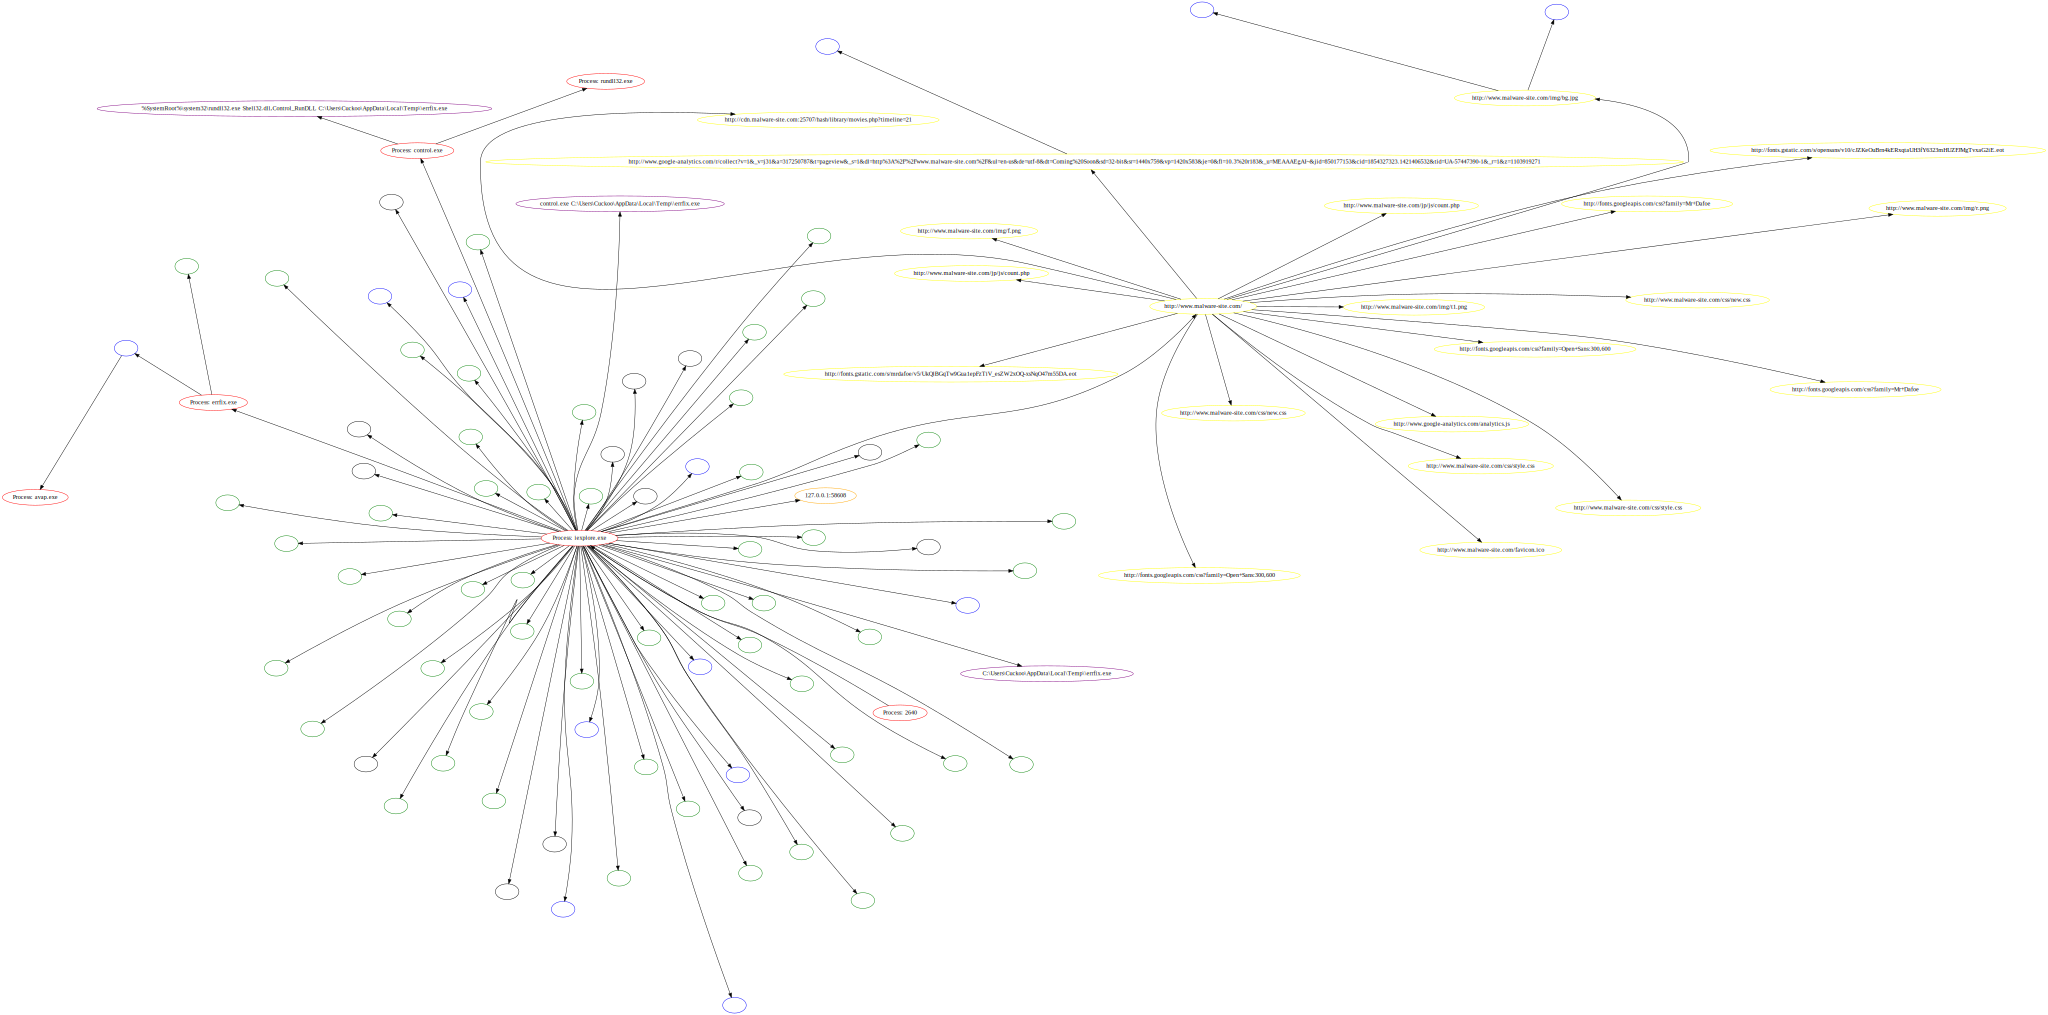
\includegraphics[width=25cm, angle=90]{Images/report_Subprocess_from_tab}
    \caption{An example of the subgraph where a single website was responsible for malware. For clarity, only the labels of visited URLs, involved processes and executed shell commands are shown.}
    \label{fig:subgraph}
\end{figure}

\stepcounter{savepage}
\pagebreak

\restoregeometry
\pagenumbering{arabic}
\setcounter{page}{\thesavepage}

\subsection{Comparison with other malware analysis systems}

To quantify the improvement that was made, several benchmarks were run against our improved version, henceforth called ``Roadrunner''\footnote{http://en.wikipedia.org/wiki/Geococcyx}. Those benchmarks were compared with a development version of Cuckoo 1.2\footnote{\url{https://github.com/cuckoobox/cuckoo/commit/6177071cfd57500fbf1dc17a66f5aff39051c75e}} and Anubis\footnote{\url{http://anubis.iseclab.org/?action=advanced\_form}}, two malware analysis systems which visit URLs sequentially.% The development version of Cuckoo was also used as the base for our development.<-- dit is niet de goeie plaats om dat te zeggen....

The benchmark, for the unmodified Cuckoo, consists of provisioning Cuckoo with one or more URLs until Cuckoo changes the status to ``reported''. Because Roadrunner does not have this status, the benchmark stops when the \texttt{mass-analyse.py} script exits. Anubis reports contain a parameter called ``time needed'' which was used as the benchmark time.

For Roadrunner, benchmarks were executed with 1, 5, 10, 25, 50 and 100 URLs and each benchmark was run 25 times to filter out anomalities. If the benchmark crashed (or hit the critical time-out) the measurement was thrown away as this is a known issue\footnote{The monitor component of Cuckoo is under active development and a significant upgrade is expected in the coming months.}, but no easy workaround was available.  Cuckoo and Anubis were both run 25 times, each with a different URL. Because both only run one URL at a given time, there is no real use in executing it with a different amount of URLs as it will be a linear increase in time with more URLs. The expected duration is calculated by multiplying the amount of URLs with the average time a single URL took.

Table \ref{tbl:results} shows the summary\footnote{The raw numbers used to generate the table and graphs can be found in Appendix B.} of the benchmarks. This table gives mean time over 25 runs of Roadrunner with the amount of URLs. For Cuckoo and Anubis, the mean of the 25 runs with 1 URL was calculated and extrapolated to higher URL counts. A comparison in the speed between Cuckoo and Roadrunner has also been made. Although the difference is significant, a important sidenote must be made that speed is not the primary goal of Cuckoo and that Cuckoo, if wanted, can be speeded up by configuration tweaks. The changes made to speedup the proof of concept removed a lot of the detailed insights Cuckoo gives in the behaviour of malware. For this project, however, only the data that makes it possible to detect malicious activity is of importance, not detailed insight of the exact behaviour of malware.

Figure \ref{fig:chart-box} and figure \ref{fig:chart-trend} show these numbers in a different way. Figure \ref{fig:chart-box} shows the boxplots of the different runs. We can say that for a higher amount of URLs, there's bigger variance in the time it takes to complete. It was not expected this would result in such (relatively) big spreading and there is no satisfactorily explanation for this behaviour. The expected result was that the differences between websites would even out on higher URL counts. Figure \ref{fig:chart-trend} is a visual representation of table \ref{tbl:results}, on the x-axis we see the number of URLs; the y-axis the time it takes to analyse these URLs. 

\setcounter{savepage}{\arabic{page}}
\stepcounter{savepage}
\pagebreak

\pagenumbering{gobble}
\newgeometry{left=3cm,top=2.5cm,bottom=0.1cm}

\begin{figure}[h!]
    \centering
    \centerline{\includegraphics[width=15cm]{Images/chart-box.png}}
    \caption{A boxplot of the benchmark durations. A higher URL count results in a higher variance of the duration.}
    \label{fig:chart-box}
\end{figure}

\begin{table}[h]
\begin{tabular}{@{}lllllll@{}}
\toprule
                                  & 1 URL    & 5 URLs   & 10 URLs      & 25 URLs      & 50 URLs     & 100 URLs \\ \midrule
Anubis       & 273,8s   & 1369,2s   & 2738,4s      & 6846,0s      & 13692,0s     & 27384,0s \\                                  
Cuckoo       & 152,8s   & 764,1s   & 1528,2s      & 3820,5s      & 7640,9s     & 15281,8s \\
Roadrunner& 48,8s    & 74,8s    & 102,4s       & 160,1s       & 286,4s      & 450,9s   \\
Improvement(\%)                   & 313,1\%  & 1021,5\% & 1492,4\%     & 2386,3\%     & 2667,9\%    & 3389,2\% \\ \bottomrule
\end{tabular}
\caption{Mean runtime of Cuckoo, Roadrunner and Anubis. Time in seconds. The improvement is calculated against Cuckoo.}
\label{tbl:results}
\end{table}

\begin{figure}[h!]
    \centering
    \centerline{\includegraphics[width=15cm]{Images/chart-trend}}
    \caption{A line chart with the results of the benchmarks. To give an indication how long it would take for higher amounts of URLs, the data has been extrapolated for up to 1000 URLs. Roadrunner is in all cases faster than both existing systems which run sequentially.}
    \label{fig:chart-trend}
\end{figure}

\stepcounter{savepage}
\pagebreak

\restoregeometry
\pagenumbering{arabic}
\setcounter{page}{\thesavepage}


\clearpage

\section{Conclusion}
This research project focused on the question how the detection of drive-by downloads can be improved by the means of concurrently visiting multiple URLs whilst still being able to determine which URL was responsible for malicious activities. To reach this goal four subquestions have been formulated and answered.

Browsers all implement the ability to concurrently visit multiple URLs in a different way. Some browsers decided to use multiple threads in a single process, but most modern browsers use subprocesses dedicated to a single or a few URLs. When multiple processes are used, it depends on the implementation if that process is directly fetching the webpages or that the main process or an intermediate process is used.

How webpages are retrieved and what the involved APIs are, is highly dependent on the implementation. Two of the examined browsers use the high-level HTTP library provided by the operating system while the other browsers implement their own. Such implementations are, for example, a custom library that is independent from other components of the web browser or an implementation where the network library is tightly integrated in the browser engine.

By monitoring the API calls to the network stack and the process and thread context they are made from, an individual HTTP request can be linked to its source. While other methods are possible, with monitoring, no modifications to the web browser are required while still all information is available.

Additional information that can be used to detect the malicious behaviour includes process, file, registry and other network related API calls. While information sources like network sniffing, syscall observation and other passive techniques could be used, no additional information would be gained.\todo{dat we hebben we wel niet in de tekst gezegd}

Based on this research, this paper proposes an algorithm that enables the possibility to do large-scale drive-by download detection by concurrently visiting multiple URLs whilst still being able to determine the responsible URL for the observed malicious behaviour.\todo{Moet er een regel in over hoe het algoritme werkt?} To validate the working and effectiveness of this algorithm, a proof of concept has been developed for an existing solution for the detection of drive-by downloads. A performance gain of 1639\% for 25 URLs has been observed.


\clearpage

\section{Future work}
Our study focused on finding a generic algorithm which allows for large-scale detection of drive-by downloads. Currently, the analysis phase is done after processing the events and creating the graph. Real-time analysis on the graph would allow for faster detection and reporting but might have more overhead. The optimal time to analyze a graph should be investigated.\\

During the proof of concept, an abstraction was made from low-level API calls to high-level events. While this greatly reduces the effort needed to analyze the graph, this poses a risk that crucial information might be missed. Further effort should be invested in finding an optimal granularity for the graph.

% Alles over de implementatie van het algoritme boeit niet, dat is niet waarover onze paper gaat
% detecting malware/drive-by downloads is dus niet echt future work


\clearpage

\section*{Acknowledgements}
\addcontentsline{toc}{section}{Acknowledgements}

First and foremost, we would like to thank our supervisors, Jop van der Lelie and Wouter Katz from the Dutch National Cyber Security Center, for the support and insight they have given during our research project. They have gravely improved the quality of this report.

We would also like to thank the Cuckoo developers (especially Jurriaan Bremer) who helped us demystify the inner workings of Cuckoo and even helped us resolving the bugs we introduced ourselves during this project.

\clearpage

\todo{Cites consistent maken}

\addcontentsline{toc}{section}{References}
\bibliographystyle{abbrv}
\bibliography{report}

\clearpage

\section*{Appendix A: Simple Analyser}
\addcontentsline{toc}{section}{Appendix A: Simple Analyser}

To implement step 3 of the algorithm a very simple analyser was written which detects a process spawn beneath tab processes. Although the real code\footnote{\url{https://github.com/MartijnB/cuckoo/blob/multi-url/utils/mass-analyse.py}} is a bit unclear, it is the same as the pseudo code in listing \ref{analysercode}.

\begin{lstlisting}[caption={Pseudo code for phase 3 of the algorithm},label={analysercode}]
function deep_process_spawn_analyser(graph)
    foreach vertex in graph
        if vertex.type == "process_spawned"
            if check_depth_in_graph(vertex, 0) > 1
                print "Malicious activity"
            endif
        endif
    endforeach
endfunction

function check_depth_in_graph(vertex, current_depth)
    parents = get_parents_of_vertex(vertex)
    # Actually we need only one parent
    if length_array(parents) > 0
        return check_depth_in_graph(parents[0], current_depth++)
    else
        # No more parents, we're at the root node
        return current_depth
    endif
endfunction
\end{lstlisting}

\clearpage

\section*{Appendix B: Raw benchmark data}
\addcontentsline{toc}{section}{Appendix B: Raw benchmark data}

\todo{Omschrijving toevoegen}

\begin{table}[h]
\begin{tabular}{@{}llllllll@{}}
\toprule
Anubis  & Cuckoo  & 1 URL       & 5 URLs      & 10 URLs      & 25 URLs      & 50 URLs      & 100 URLs     \\ \midrule
260,0s  & 148,5s  & 44,8s       & 93,7s       & 109,3s       & 144,2s       & 271,0s       & 455,9s        \\
311,0s  & 161,2s  & 45,2s       & 85,3s       & 100,4s       & 140,5s       & 240,3s       & 431,9s        \\
267,0s  & 152,2s  & 45,2s       & 67,7s       & 84,0s        & 152,2s       & 251,8s       & 438,8s        \\
299,0s  & 152,1s  & 47,1s       & 59,9s       & 86,9s        & 146,0s       & 272,2s       & 456,9s        \\
283,0s  & 143,4s  & 44,9s       & 67,6s       & 141,0s       & 156,4s       & 254,7s       & 482,3s        \\
271,0s  & 149,5s  & 43,8s       & 83,5s       & 100,8s       & 155,7s       & 252,3s       & 414,2s        \\
270,0s  & 152,9s  & 46,2s       & 74,8s       & 90,0s        & 138,4s       & 247,9s       & 480,1s        \\
250,0s  & 146,0s  & 44,7s       & 65,1s       & 135,1s       & 153,5s       & 240,7s       & 430,7s        \\
282,0s  & 159,0s  & 47,8s       & 92,5s       & 87,2s        & 161,5s       & 257,5s       & 410,6s        \\
265,0s  & 148,3s  & 60,0s       & 63,9s       & 93,5s        & 172,8s       & 297,0s       & 429,2s        \\
251,0s  & 153,5s  & 47,0s       & 76,4s       & 103,4s       & 185,4s       & 248,3s       & 452,5s        \\
264,0s  & 147,9s  & 47,6s       & 106,5s      & 90,0s        & 144,1s       & 265,3s       & 442,3s        \\
264,0s  & 160,7s  & 52,5s       & 74,4s       & 128,0s       & 156,0s       & 582,7s       & 537,1s        \\
279,0s  & 152,3s  & 51,3s       & 64,8s       & 95,7s        & 156,8s       & 265,4s       & 461,4s        \\
255,0s  & 144,0s  & 61,7s       & 65,9s       & 84,2s        & 160,3s       & 251,6s       & 441,2s        \\
357,0s  & 146,8s  & 45,8s       & 104,3s      & 109,1s       & 163,9s       & 261,5s       & 436,1s        \\
251,0s  & 164,3s  & 46,2s       & 69,7s       & 86,4s        & 166,9s       & 253,3s       & 438,3s        \\
279,0s  & 148,6s  & 46,9s       & 68,1s       & 103,5s       & 145,9s       & 332,1s       & 465,9s        \\
275,0s  & 152,5s  & 48,3s       & 69,6s       & 88,0s        & 185,9s       & 535,8s       & 409,4s        \\
265,0s  & 146,2s  & 61,2s       & 65,5s       & 93,3s        & 175,4s       & 258,9s       & 463,5s        \\
298,0s  & 148,1s  & 54,1s       & 70,6s       & 138,8s       & 202,8s       & 259,4s       & 466,5s        \\
256,0s  & 185,5s  & 45,7s       & 67,0s       & 104,7s       & 186,5s       & 284,9s       & 481,0s        \\
256,0s  & 161,1s  & 42,7s       & 74,4s       & 110,8s       & 165,1s       & 260,2s       & 451,8s        \\
271,0s  & 144,1s  & 54,1s       & 70,4s       & 95,8s        & 139,7s       & 267,6s       & 446,4s        \\
277,0s  & 151,9s  & 45,9s       & 69,5s       & 99,8s        & 146,3s       & 247,6s       & 448,0s        \\ \bottomrule
\end{tabular}
\caption{Raw values of benchmarks in seconds.}
\label{my-label}
\end{table}

\clearpage

\section*{Appendix C: Cuckoomon modifications}
\addcontentsline{toc}{section}{Appendix C: Cuckoomon modifications}
\label{cuckoomonmods}

Cuckoomon is the analyser component of Cuckoo. It hooks interesting API functions and logs their usage. As part of the development of the proof of concept, many hooks have been disabled and several missing ones added.

\textbf{Added hooks}

\begin{longtable}{*{2}{>{\arraybackslash}p{6cm}}}
URLDownloadToFileA     & HttpSendRequestExW           \\
FtpOpenFileA           & HttpEndRequestA              \\
FtpOpenFileW           & HttpEndRequestW              \\
FtpGetFileA            & HttpQueryInfoA               \\
FtpGetFileW            & HttpQueryInfoW               \\
FtpPutFileA            & InternetConfirmZoneCrossingA \\
FtpPutFileW            & InternetConfirmZoneCrossingW \\
HttpAddRequestHeadersA & InternetReadFileExA          \\
HttpAddRequestHeadersW & InternetReadFileExW          \\
HttpSendRequestExA     &                             
\end{longtable}

\textbf{Removed hooks}

\begin{longtable}{*{2}{>{\arraybackslash}p{6cm}}}
NtReadFile            & NtDeviceIoControlFile   \\
NtQueryDirectoryFile  & NtQueryInformationFile  \\
NtOpenDirectoryObject & FindFirstFileExA        \\
FindFirstFileExW      & GetDiskFreeSpaceExA     \\
GetDiskFreeSpaceExW   & GetDiskFreeSpaceA       \\
GetDiskFreeSpaceW     & RegEnumKeyW             \\
RegEnumKeyExA         & RegEnumKeyExW           \\
RegEnumValueA         & RegEnumValueW           \\
RegQueryValueExA      & RegQueryValueExW        \\
RegQueryInfoKeyA      & RegQueryInfoKeyW        \\
NtEnumerateKey        & NtEnumerateValueKey     \\
NtQueryValueKey       & NtQueryMultipleValueKey \\
NtLoadKey             & NtLoadKey2              \\
NtLoadKeyEx           & NtQueryKey              \\
FindWindowA           & FindWindowW             \\
FindWindowExA         & FindWindowExW           \\
EnumWindows           & NtOpenMutant            \\
NtOpenSection         & ZwMapViewOfSection      \\
ExitProcess           & NtUnmapViewOfSection    \\
NtFreeVirtualMemory   & SetWindowsHookExA       \\
SetWindowsHookExW     & UnhookWindowsHookEx     \\
LdrGetDllHandle       & LdrGetProcedureAddress  \\
ExitWindowsEx         & LookupPrivilegeValueW   \\
WriteConsoleA         & WriteConsoleW           \\
GetSystemMetrics      & GetCursorPos            \\
GetComputerNameA      & GetComputerNameW        \\
GetUserNameA          & GetUserNameW            \\
NtDelayExecution      & GetLocalTime            \\
GetSystemTime         & GetTickCount            \\
NtQuerySystemTime     & send                    \\
sendto                & recv                    \\
recvfrom              & select                  \\
connect               & WSARecv                 \\
WSARecvFrom           & WSASend                 \\
WSASendTo             & CryptProtectData        \\
CryptUnprotectData    & CryptProtectMemory      \\
CryptUnprotectMemory  & CryptDecrypt            \\
CryptEncrypt          & CryptHashData           \\
CryptDecodeMessage    & CryptDecryptMessage     \\
CryptEncryptMessage   & CryptHashMessage       
\end{longtable}

\end{document}
